% HEADER Section
% Define formal of the paper
\documentclass[sigconf, natbib=false]{acmart}
\setcopyright{none} % Remove the 
\settopmatter{printacmref=false} % Removes citation information below abstract
\renewcommand\footnotetextcopyrightpermission[1]{} % removes footnote with conference information in first column
\pagestyle{plain} % removes running headers
\setlength{\marginparwidth}{2cm}
\usepackage{outlines} % item and sub items 
\usepackage{pifont} %provides addition symbols


%% Include packages 
\usepackage[style=ACM-Reference-Format,backend=bibtex,sorting=none]{biblatex}
\addbibresource{ref.bib}
\usepackage{lipsum}% for dummy text
\usepackage[parfill]{parskip} % create space between paragraph
\fancyfoot{}
\usepackage{booktabs} % For formal tables
\usepackage{subcaption}

% package for drawing flowchart 
\usetikzlibrary{shapes.geometric, arrows}
\usepackage{caption}  

% package for to do 
\usepackage{xcolor}
\newcommand\mytodo[1]{\textcolor{red}{#1}}
\usepackage{todonotes}

% packages for pseudo code 
% \usepackage{algorithm} 
% \usepackage[noend]{algpseudocode}
% \usepackage{algpseudocode}
\usepackage{algcompatible}
\usepackage[noend, ruled,lined]{algorithm2e}

% Drawing figure with tikz package
\usepackage{tikz}
\usetikzlibrary{positioning, shapes}



%table 
\usepackage{multirow}
\usepackage{graphicx}

\newcommand\MyBox[2]{
  \fbox{\lower0.75cm
    \vbox to 1.7cm{\vfil
      \hbox to 1.7cm{\hfil\parbox{1.4cm}{#1\\#2}\hfil}
      \vfil}%
  }%
}

% Paraphase, grammer 



%% Author Information 
\title{A Data-Driven Machine Learning Approach to Detect Suspicious Companies}
\author{Asif Anwar (2660561)}
\affiliation{%
  \institution{Vrije Universiteit}
  \streetaddress{ De Boelelaan 1105}
  \city{Amsterdam} 
  \country{The Netherlands} 
  \postcode{1081 HV}
  }
\email{a.anwar@student.vu.nl}


% Main report 

\begin{document}



\begin{titlepage}
    \begin{center}
    \vspace{0.8cm}
        \includegraphics[width=0.4\textwidth]{figures/vua.pdf}
        \vspace*{1cm}
        
        \Huge
        \textbf{Eagle Eye: Trade Fraud Detection Using Machine Learning Techniques}
        
        \vspace{0.5cm}
        \LARGE
        Master Thesis \\
        
        
        \vspace{2.5cm}
        \large
        Author: \\
        \vspace{0.25cm}
        \Large
        Name: \textbf{Asif Anwar}\\
        \vspace{0.25cm}
        \large
        Id: AAR216\\
        \vspace{0.25cm}
        Email: A.Anwar@student.vu.nl\\
        
        \vspace{1.5cm}
        \large
        supervisor: \\
        \vspace{0.25cm}
        \Large
        \textbf{Dr. Charlotte GerritsenDaily}
        

        
        \vfill 
        
        \today \\
        \vspace{0.5cm}
        Submitted in partial fulfillment of the requirements for\\ 
        the degree of Master of Science in Artificial Intelligence. 
        
        \vspace{1cm}
        
   
        
        \vspace{2.5cm}
        
        
    \end{center}
\end{titlepage}

\newpage
    \thispagestyle{empty}
    \tableofcontents
\newpage

\begin{abstract}
    Trade credit fraud is a major concern for suppliers and insurance companies. An accurate and effective classification method can reduce potential financial loss, as well as reduce massive operational costs for the organisations. However, due to a large amount of unstructured data and high-class imbalance, fraud classification is an enormously challenging task. The goal of this paper is to find a suitable machine learning model to identify suspicious companies. A data-driven approach has been applied to extract features and generate the required dataset. Then different machine learning techniques have been used to handle imbalance classes and build models. based on different performance matrices like ROC, AUC, confusion metrics, recall are used to find the best models and Threshold limits to fine-tune to model. Random Forest classifiers with majority class under-sampling and minority class oversampling by artificial data generated by SMOTE perform the best with the highest AUC score of 0.817. 
    
\end{abstract}
\keywords{Fraud Detection, Machine Learning, SOMTEC, Data Mining}

\maketitle
\pagestyle{plain}
\balance

% Include Sections 
\section{Introduction} \label{sec: Intro}
% This section includes some motivations behind the work, explicitly or implicitly highlights the research question , provides a high-level explanation of the solution, and describes the contributions.

% establish the context, background and/or importance of the topic
In the current global economy, the financial fraud has become a crucial issue especially for the trade sector. In recent times, the number of fraud cases have increased drastically which effected both financial institutions and their clients significantly. From a survey in 2020 on economic crime and fraud by Price Waterhouse Coopers, its been reported that more than 42 billion USD of financial losses happened in past 24 months~\cite{PwC.Crime.Survey}. On an average companies reportedly experienced 6 fraud cases during this period. Thirty five percent of fraud cases are marked as Customer fraud~\cite{PwC.Crime.Survey}.   

In current trend, more and more, companies outsource non-core activities to third party companies to reduce operational costs. But these third party-party business partners can be fraught with risk. One in five respondents from the PwC survey~\cite{PwC.Crime.Survey} cited vendors/suppliers as the source of their most disruptive external fraud. On the other hand, suppliers are also in high risk of fraud cases from their buyers. Due to this detecting suspicious companies (buyers and suppliers) plays an important role to reduce financial losses for the trade insurance companies and theirs customers.



% brief synopsis of the relevant literature
Fraud or extortion is a par of internal threats for any business. Manufacturers and service providers may face financial losses from fraudulent buyers. According to Association of Certified Fraud Examiners ACFE, the definition of fraud is \"the use of one’s occupation for personal enrichment through the misuse or deliberate
misapplication of the resources or assets of the employing organization~\cite{kassem_2014}. To term fraud that is imposes to manufactures and service provider it can be redefined as the personal gain of the buyers by misuse or deliberate misapplication of the products and services of the supplying organization and their respective insurance companies.

\begin{figure}[htp]
    \centering
    \includegraphics[width=\linewidth]{figures/fraud_by_industry.PNG}
    \caption{Most disruptive fraud events – by industry.Source: PwC 2020 Fraud survery~\cite{PwC.Crime.Survey} }
    \label{fig:fraud_sector}
\end{figure}
% Indicate an issue, problem or controversy in the field of study

A classical approach to prevent such fraudulent cases is done by traditional method of using human resources like internal and external auditors~\cite{kassem_2014}, and business team. Each team has their own process of monitoring external partners and buyers by analyzing transaction patterns, financial overview, historical behaviour to identify suspicious companies.  Based on the organizational capabilities, these team uses different internal and external resources like archival system, reports and news source.


Historically, organizations and financial institutions are using different technological solutions and operational process to detect suspicious companies. In the technological solutions different software are used to verify names, previous history and financial status of the buyers. On the other hand, as part of operational process during the customer on-boarding the Know Your Customer KYC process are used to identify anomaly in the customer profile. However, the major problems for these existing solution to detect suspicious companies are complex, time consuming, costly,and cognitively challenging labour intensive task.


However, in recent past with the advancement of artificial intelligence and data mining techniques, different machine leaning solutions are developed to find anomalies, credit card fraud, etc.~\cite{RB2021, KIRKOS2007995}. Considering the complexity of the tasks the continuous improvement of the systems are going on. The incremental success of these solutions are showing a great promises to reduce operations time and cost for the organizations and financial institutions.

Most studies in the field of suspicious activity classification for economical sector are done on Credit Card fraud detection. The recent number of individual and organized criminals the number of credit card has increased significantly ~\cite{RB2021}. Although lots of research has been carried out on detecting anomalies in financial crime, we can see that most of the researches for identifying suspicious financial crime activity are focused on detecting credit card fraud. However, as mentioned earlier, in the survey from PwC we have seen that third party business crime and fraud imposes high risk and have huge financial impact on the economy.
% listing the reasarch question or hypotheses


This paper will focus on using a data-driven approach using machine learning techniques to detect suspicious companies to prevent financial losses for the organizations and respective financial institutions.  The major objective of this study is to use data mining technique to extract features from unstructured data, and apply ensemble learning and neural network to identify the pattern on the features to detect suspicious companies.

% provide synopsis of the research methols



Data extracted is a useful method to gather data for analysing and prediction tasks. Data driven is a method base on the history data to build more hyper-parameters to compensate the un-measurable features within the measurable data \cite{SMARRA20181252}. some extending nonlinear features to build the prediction function. In classification and prediction problem, it is essential to discover the pattern of the data and provide us some insights to take some actions according to the prediction results. Random Forest algorithm and Neural Networks are been used in handling this problem and shown effective~\cite{10.1145/3414274.3414278, RB2021}. However it is extremely hard to identify the target information from institutions data based on pattern. The propose of the paper is to find a suitable classifier and its application to find fraudulent cases based on assembly learning and machine learning .

\mytodo{update this text}



% Significance of value of the study


This thesis provided an important opportunity to advance the understanding of data-driven approach for extrapolate data from historical archive based on expert opinion. Also the paper covers how a real-world data with high class imbalanced is used for different machine learning approaches. The paper also tries to explain the complexity and challenges of identifying anomalies in the data set and share a practical overview on how to approach suspicious recommendation engine can be applied this financial and other suitable sectors.



% Define the topic or key term


Throughout this paper, the term Artificial Neural Networks, Random Forest, XGBoost, receiver operating characteristic, and are under the curve will refer to ANN, RF, XG, ROC and AUC. The term fraud is used interchangeably with suspicious activity done by companies to gain financial gain.

% Overview of teh report stucture


The main question address in this paper are:
\begin{itemize}
    \item[a.] Data driven approach to extract relevant information related to detecting suspicious behaviour or patters of companies
    \item[b.] Choosing the most appropriate model for detecting suspicious companies to prevent fraudulent cases.
\end{itemize}

To overall structure of the design takes the form of three steps. In step 1 a data driven technique is used to identify the most significant information based on the feedback from expert then extracting the information from historical dataset. In step 2 ensemble models and neural networks are used for suspicious companies classification problem. And last but not least, in step 3 Different machine learning metrics are used to select the best performing model. The details of the approach are described in the overview [section: ~\ref{sec: Overview}] and design [sec:~\ref{sec: Design}] section of this paper.
% State the purpose of the essay / write


The case study of identifying suspicious companies that presented in this paper is conducted for one of the leading trade insurance company. The interested company has foot print over different locations in the world. The target of the company to reduce risk by preparing a classification model which recommends or detects suspicious companies to prevent itself from having financial loss due to fraudulent activity.
% Provide an overview of the coverage


Designing and setting the suitable machine learning model is a repetitive process. In this paper only section method of first model is described. Due to practical constrain not all other machine learning models and configuration of assembly models and neural networks are discussed. Also due to protect the internal process of the expertise of the insurance company have been excluded while describing the feature. However in the design section a generalized approach and pseudo code have been shared in section:~\ref{sec: Design}]







\section{Background} \label{sec: background}
% This section provides the necessary context to help the reader understand the remainder of the thesis.

% Why this report is generated

The aim of this paper is to perform a data driven approach to extract relevant data to build machine learning classification model to detect specious company for a leading trade credit insurance provider. The trade credit insurance provides protection to the business (customer of the insurance company) in the event their buyers fail to pay for the products or services. Considering the raise of fraudulence business in recent past, the insurance provider has to monitor each buyers extensively before approving any insurance policy. Considering the number of number of policies are so high, a machine learning based recommended system was implemented for UK market to detect suspicious companies. Since the implementation of the system the solution saved around 1M pounds. Due to the success of the UK model, the organization decided to implement similar recommendation ending in other market.

For this paper, the a model focuses on identifying suspicious companies for Italian Market. Each country is fundamentally different in terms of trade credit policy. Hence, each country has its own internal process and method to identify the suspicious cases. To build the recommendation model below data driven machine learning strategies are used.

\mytodo{update terms: buyers, client and provider}

\subsection{Trade Credit Insurance}\label{subsec:trade-credit-insurance}
In business world trade credit is a regular practice done by manufactures, suppliers, and service providers to protect their financial interest from any types of risks.\mytodo{find the total yearly trade credit amount}. Companies sales their products and goods on credit to their buyers. Generally this is a continues process as back to back trade deals and payment happens between the suppliers and buyers. However, the amount of trade credit is very high, hence suppliers like to protect their interest by taking credit polices from financial institutions  \mytodo{cite what is trade credit}.

For financial institutions (credit insurance provider) ensures financial support to the supplier (client) in event of any mishaps. Trade credit is a risky business, hence before providing any insurance, financial institutions verifies both both supplier, sales, global economic conditions, external factors. As mentioned in section~\ref{sec: Intro}, due to the increased number of fraud cases, insurance providers have to also monitor fraudulent cases. Below are the types of fraud happens in the trade credit sector.

\begin{itemize}
    \item \textbf{Buyers Fraud:} When the buyers of the goods and products get benefited by not paying the dues to the suppliers.
    \item \textbf{Client Fraud:} When the clients of the insurance company, suppliers try to gain benefit by doing insurance fraud.
    \item \textbf{Joint Fraud:} When the suppliers and buyers cooperate another do conduct insurance fraud.
    \item \textbf{Internal Fraud:} When internal parties from the insurance company colludes with the client and conduct an insurance fraud.
\end{itemize}

In this study we will mainly focus on finding the suspicious buyers to prevent economic mishaps to protect the suppliers and the insurance companies from financial loss.


\subsection{Monitor Credit Policy}\label{subsec:monitor-credit-policy}


In the the figure~\ref{fig:trade_credit}, the process of trade credit issuance is shown.

\begin{figure}[htp]
    \centering
    \includegraphics[width=\linewidth]{figures/monitor_buyers.jpg}
    \caption{Trade credit issuing process}
    \label{fig:trade_credit}
\end{figure}

\subsubsection{Traditional Approach}

\subsubsection{Machine learning base Approach}




\section{Related Work}\label{sec:related-work}

Some of the related studies done by various researchers are highlighted in this section. These researches are on different types of machine learning techniques and various methods for data mining and prepossessing techniques. The main recherche topics are focused on finding fraudulent transactions or even using machine learning methods. 


Asha RB and Suresh Kumar KR proposed a method to detect the fraud in credit card transactions that are based on deep learning \cite{GoodBengCour16} in the paper credit card fraud detection using artificial neural network \cite{RB2021}. Frauds in credit card transactions are the most common and frequent issue. In the paper the researcher usages support vector machine (SVM) \cite{Cristianini2008}, k-nearest neighbour (KNN) \cite{Mucherino2009} and artificial neural network (ANN). The paper concludes that an artificial neural network (ANN) gives an accuracy of 0.99 with a precision of 0.81 and a recall of 0.76.



Class imbalance is one of the major challenges for classifying fraudulent cases. In the paper "Deep Over-sampling Framework for Classifying Imbalanced Data" \cite{ando2017deep} Shin Ando and Chun Yuan Huang have proposed a framework that extends the synthetic over-sampling method to the deep feature space acquired by a convolutional neural network (CNN) \cite{Yamashita2018}. Deep Over-sampling uses the overloaded instances to supplement the minority classes.  


In the paper "Data Mining techniques for the detection of fraudulent financial statements" \cite{KIRKOS2007995}, Efstathios Kirkos, Charalambos Spathis, and Yannis Manolopoulos explore the effectiveness of Data Mining (DM) classification techniques in detecting firms that issue fraudulent financial statements. Data Mining proposes several classification methods derived from the fields of statistics and artificial intelligence. As per the research three methods, which enjoy a good reputation for their classification capabilities


Kamat Nath Mishra and Subhash Chandra proposed a k-fold machine learning techniques for fraud prediction in smart societies \cite{Mishra2021}. In their paper on fraud detection, they have classified the types of credit card fraud types. They proposed a logistic regression-based solution. The implementation of their methodology is then further analysed using machine learning tools like ROC curve \cite{FAWCETT2006861}, confusion matrix, mean-recall score value and precision-recall curve. 


In the paper "Imbalanced Classification Problem Using Data-driven and Random Frost Method" \cite{10.1145/3414274.3414278} the researcher Wan Wang, Xinglu Liu and Victor Chan proposed a classification method for an imbalanced dataset using data-driven technique and random forest. The research is done over three open-source datasets. The result shows that random forest applied with a data-driven approach improved the prediction accuracy. The AUC values also perform well stable and even increased. The researcher augured that they used an imbalanced dataset that represent real-world data. So in theory their approach should perform reasonably in real-world scenarios. 



Important insights for selecting machine learning algorithm for skewed dataset has been discussed in the paper "The relationship between precision-recall and ROC curves" \cite{davis06}. As per the researcher Jass Davis and Mark Goadrich, ROC space and PR space have a deep connection. When a curve dominates in ROC space it also dominates in PR space. They also shared that a model which optimised the area under the ROC curve is not guaranteed to optimise the area under the PR curve. This study can be really handy for our use case of fraud detection. 


In The literature review named "Fraud detection using the fraud triangle theory and data mining techniques" \cite{computers10100121} the researchers highlighted the complexity of predicting Fraud. They explained the human behavioural aspect of fraudulent activity and how traditionally detection was performed by auditors and manual technologies. The researcher mentioned in the paper, in the recent past how several works related to fraud detection using machine-learning techniques were identified without the evidence that they incorporated the fraud triangle as a method for more efficient analysis. \label{sec: related work}
\section{Overview}\label{sec: Overview}
% This section provides a high-level outline of the proposed system or solution. It typically illustrates the system architecture or the interactions between the different solution components (via a “boxes-and-arrows” diagram) from a user’s perspective.

\mytodo{intro chapter on Overall design}

A joint data-driven technique and machine learning algorithms approach are used in this work for this classification task. Before the classification step, number of new features are generated or engineered from the internal company data. the insight from the experts are considered first, then from the historical reports the data driven method was used to prepare a dataset to train the desired model. Based on statistical correlation the important features are selected as final features to train various Ensemble models and artificial neural networks are used to get the best out come. \mytodo{refer the the three step flow}

Firs step of data driven approach is to apply the theory of change. As per the theory of change we can find the road map for how to get company information which are most useful. This method also help to find how to archive long time goals along with indicator for improve and track progress. Then its important to get in touch with internal experts to understand what sort of data they are using for daily tasks.

Generally the classifiers perform quite weak due to missing values and imbalance dataset for real life scenarios. The one of the major reason for the missing data is the collected data does not contain enough information, because of he statistical error or some missing values. To obtain more hidden
information, data-driven method generally is a good choice. In the data driven approach hidden features can be found based on feedback from expert

Data-driven decision making means getting the right data to the right model to the right time to improve the model for problem solving. This approach can help the organisation to identify and apply recent trend in data to apply it for finding solutions.

\subsection{Proposed architect}\label{subsec:propsed-architech}
\mytodo{fill architect section}
\begin{figure}[htp]
    \centering
    \includegraphics[width=\linewidth]{figures/overall_design.PNG}
    \caption{Overall Design}
    \label{fig:design}
\end{figure}

\mytodo{highlight the coverage in this paper}

\subsection{Imbalance Class Problem}\label{subsec:imbalance-class-problem}
Training classification model using imbalance data set generally leads to bias to predict one sample from another. Considering the fraudulent or suspicious number of companies are so less, the training data set for fraud detection is highly imbalanced. Before training the classifier, the data set can be fixed by using below sampling methods.    
\subsubsection{Under-sampling:}\hspace*{\fill} \\
Under sampling is one of the common and basic method of sampling to reduce class biases \cite{10.1145/3055635.3056643}. In this method a selective number of (generally equal number of smaller class data) samples are taken from large class. The samples are randomly taken and number of instances are based on minority class. This method provide the smaller dataset than the actual one as the number of instances for majority class reduces dramatically. 
\subsubsection{Over-sampling}\hspace*{\fill} \\
For over sampling method, the more samples are taken from the minority class so that the main dataset becomes balanced. Even though the random sampling method is used for taking samples, but due to class imbalance, we can see that number of repeated instances are copied from the minority class to prepare the dataset. This method provide the larger dataset as the number of instances for minority class increases. 

\subsubsection{SMOTE}\hspace*{\fill} \\
SMOTE is a synthetic over sampling method \cite{2002}. SMOTE drastically improve the performance of classifying minatory class by creating synthetic samples. Generally the synthetic samples are randomly generated by randomly selected minority class samples with interpolation between the neighbours of the selected sample. SMOTE facilitate balanced dataset with related minority class samples to learn from, which allows the models to decision boarder regions,  leading coverage of the minority class.

\subsubsection{Combined Sampling}\hspace*{\fill} \\
In the combined sampling method two or more samplings method are used in the same data set \cite{10.1145/3055635.3056643}. Under and over sampling is a common approach. In this method the under-sampling of majority class and over-sampling of minority class are done to prepare the Dataset. Another suitable method is to under-sample the majority class and synthetic sampling minority class. 

% Source from paper 31
\subsection{Model Selection}\label{subsec:model-selection}

\subsection{Ensemble learning}\label{subsec:ensemble-learning}\hspace*{\fill} \\
As they use a collection of results to make a final decision, they are referred to as ensemble techniques.
\mytodo{small about ensemble learning}

\begin{outline}
 \1 \textbf{Random Forests:} Random forest classified is designed based on decision tree A is a decision tree in classification tree which each node has a  decision based on binary whether  $x_i < \alpha$ or $\alpha$  not for a fixed. The random forests classifiers are a combination of large number of decision tree  algorithms \cite{breiman2001random} ensemble together. Random forest algorithm is designed in a such a way that it combines a large number of relatively uncorrelated decision tress \cite{breiman2001random}. The random forest performs better than a singe decision tree specially to handling over-fitting and under-fitting for the training set \cite{Mishra2021}. The performance of the random forest algorithm depends on the strength of the individual tress in the forest and the correlation between them. This algorithm also introduce feature randomness by picking up only from a random subset of features which allows it to perform better with classification without over-fitting the training data set. Random forest constructed many individual decision tress at training. Prediction from all trees are pooled to make the final prediction; the mode of the classes for classification.  
 
 \2 Feature Importance: Feature importance is defined based on the probability of finding that particular node. The probability is calculated by ratio of samples reach that node. The higher value gets more importance in feature space. 
 
 \2 Gini Impurity: Gini impurity is used for classification tasks. $\sum_{i=1}^{C} f_i{(1-f_i)}$, \textbf{$f_i$} is the frequency of label i at a node and \textbf{C} is the number of unique labels. 
 
 \2 Information gain: Information gain is used for splitting the data using entropy. This is calculated as the change in entropy after the dataset split on an attribute. $Gain(T,X) = Entropy(T) - Entropy(T,X)$, here \textbf{T} is target variable, \textbf{X} is the feature to be split on \textbf{Entropy(T,X)} which is calculated after the data is split on feature. \mytodo{cite}
 
 $$ni_j =w_jC_j - w_{left(j)}C_{left(j)} - w_{right(j)}C_{right(j)}$$
 

 %\cite https://towardsdatascience.com/the-mathematics-of-decision-trees-random-forest-and-feature-importance-in-scikit-learn-and-spark-f2861df67e3%
 
 \1 \textbf{XGBoost:} XGBoost is an ensemble method with the main goal of reducing bias and variance. Gradient boosting which employs the gradient descent algorithm to minimise loss \cite{Chen:2016:XST:2939672.2939785}. The algorithm forms trees sequentially and each new tree aims to reduce the error of the previous tree (10). The feature weights are readjusted and each new tree learns from its ancestors and the residual error is updated. A strong model is formed by combining successive weak learners which have high bias to make the final prediction thus reducing both bias and variance.
\end{outline}




\subsubsection{Neural Network}
\mytodo{briefing about neural network}
\tikzset{%
  every neuron/.style={
    circle,
    draw,
    minimum size=0.5cm
  },
  neuron missing/.style={
    draw=none, 
    scale=2,
    text height=0.333cm,
    execute at begin node=\color{black}$\vdots$
  },
}

\begin{figure}[h]
    \centering
        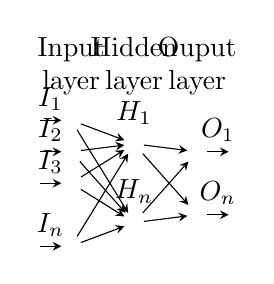
\begin{tikzpicture}[x=.4cm, y=0.4cm, >=stealth]
        
            \foreach \m/\l [count=\y] in {1,2,3,missing,4}
              \node [every neuron/.try, neuron \m/.try] (input-\m) at (0,2.5-\y) {};
            
            \foreach \m [count=\y] in {1,missing,2}
              \node [every neuron/.try, neuron \m/.try ] (hidden-\m) at (2,2-\y*1.25) {};
            
            \foreach \m [count=\y] in {1,missing,2}
              \node [every neuron/.try, neuron \m/.try ] (output-\m) at (4,1.5-\y) {};
            
            \foreach \l [count=\i] in {1,2,3,n}
              \draw [<-] (input-\i) -- ++(-1,0)
                node [above, midway] {$I_\l$};
            
            \foreach \l [count=\i] in {1,n}
              \node [above] at (hidden-\i.north) {$H_\l$};
            
            \foreach \l [count=\i] in {1,n}
              \draw [->] (output-\i) -- ++(1,0)
                node [above, midway] {$O_\l$};
            
            \foreach \i in {1,...,4}
              \foreach \j in {1,...,2}
                \draw [->] (input-\i) -- (hidden-\j);
            
            \foreach \i in {1,...,2}
              \foreach \j in {1,...,2}
                \draw [->] (hidden-\i) -- (output-\j);
            
            \foreach \l [count=\x from 0] in {Input, Hidden, Ouput}
              \node [align=center, above] at (\x*2,2) {\l \\ layer};
        
        \end{tikzpicture}
    \caption{Neural Network}
    \label{fig:neural network}
\end{figure}

\begin{outline}
 \1 Activation functions 
   \2 Sigmoid: label/multi-label binary classification. in equation \ref{eq:sigmoid}
   \2 relu: 
 \1 Loss Functions
    \2 Cross Entropy: In binary classification, where the number of classes \textbf{M} equals 2, Binary Cross-Entropy(BCE) can be calculated as shown in equation \ref{eq:Cross Entropy}. 
 \1 Optimiser
    \2 Adam: Adaptive Moment Estimation (Adam) [14] is another method that computes adaptive learning rates for each parameter. In addition to storing an exponentially decaying average of past squared gradients vt like Adadelta and RMSprop, Adam also keeps an exponentially decaying average of past gradients mt, similar to momentum. Whereas momentum can be seen as a ball running down a slope, Adam behaves like a heavy ball with friction, which thus prefers flat minima in the error surface $m_n = E[X^n]$, here $m$ is momentum and $X$ is a random variable. 
 \1 Regularisation
    \2 L1: A regression model that uses L1 regularisation technique is called Lasso Regression. \ref{eq:L1}
    \2 L2: A regression model that uses L2 regularisation technique is called Ridge Regression. \ref{eq:L2}

\end{outline}


\begin{equation} \label{eq:sigmoid}
    Sigmoid: \sigma(z) = \frac{1} {1 + e^{-z}}
\end{equation}

\begin{equation} \label{eq:Relu}
    Relu(z) = max(0, z)
\end{equation}


\begin{equation} \label{eq:Cross Entropy}
   Cross Entropy Loss: -{(y\log(p) + (1 - y)\log(1 - p))}
\end{equation}

\begin{equation} \label{eq:L1}
    L1: Loss = Error(Y - \widehat{Y}) + \lambda \sum_1^n |w_i|
\end{equation}

\begin{equation} \label{eq:L2}
    L2: Loss = Error(Y - \widehat{Y}) +  \lambda \sum_1^n w_i^{2}
\end{equation}

\subsection{Tools of Trade}\label{subsec:tools-of-trade}

\subsubsection{Receiver Operating Characteristic (ROC):}\hspace*{\fill} \\
Receiver operating characteristics (ROC) graphs are useful for organising classifiers and visualising their performance. ROC graphs are commonly used in medical decision making, and in recent years have been used increasingly in machine learning and data mining research. Although ROC graphs are apparently simple, there are some common misconceptions and pitfalls when using them in practice. The purpose of this article is to serve as an introduction to ROC graphs and as a guide for using them in research. \cite{FAWCETT2006861}

\subsubsection{Confusion Matrix:}\hspace*{\fill} \\
A confusion matrix is a tool to visualise the performance of the classifier in a matrix form \cite{Ting2017}. In a confusion matrix the true classes of the object and the prediction of the classifiers are presented in a two-dimensional matrix. For binary classification problem, confusion matrix is a widely used tool as it gives a clear view of the performance of the classifiers. 

\begin{equation} \label{eq:aqquracy}
    Accuracy = \frac{TP+TN}{TP+TN+FP+FN}
\end{equation}

\begin{equation} \label{eq:precision}
    Precision = \frac{TP}{TP+FP}
\end{equation}

\begin{equation} \label{eq:recall}
    Recall = \frac{TP}{TP+FN}
\end{equation}


\begin{table}[]

    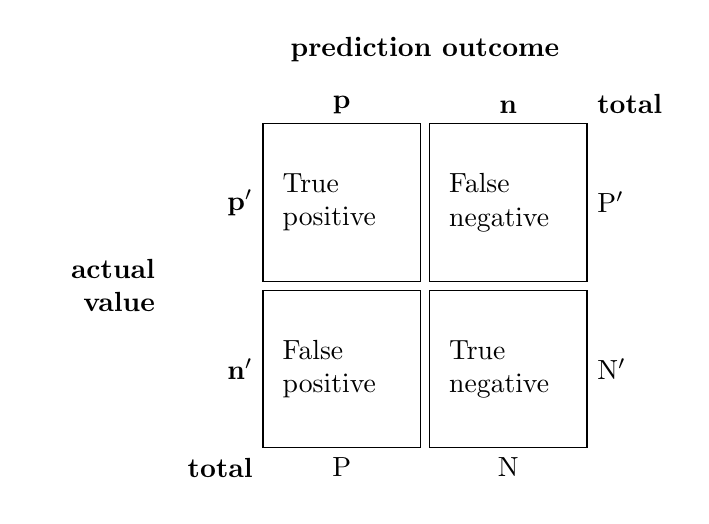
\begin{tikzpicture}[
        box/.style={draw,rectangle,minimum size=2cm,text width=1.5cm,align=left}]
        \matrix (conmat) [row sep=.1cm,column sep=.1cm] {
        \node (tpos) [box,
            label=left:\( \mathbf{p'} \),
            label=above:\( \mathbf{p} \),
            ] {True \\ positive};
        &
        \node (fneg) [box,
            label=above:\textbf{n},
            label=above right:\textbf{total},
            label=right:\( \mathrm{P}' \)] {False \\ negative};
        \\
        \node (fpos) [box,
            label=left:\( \mathbf{n'} \),
            label=below left:\textbf{total},
            label=below:P] {False \\ positive};
        &
        \node (tneg) [box,
            label=right:\( \mathrm{N}' \),
            label=below:N] {True \\ negative};
        \\
        };
        \node [left=.05cm of conmat,text width=1.5cm,align=right] {\textbf{actual \\ value}};
        \node [above=.05cm of conmat] {\textbf{prediction outcome}};
    \end{tikzpicture}

    
    \caption{Confusion Matrix}
    \label{tab:Confusion Matrix}
\end{table}
\mytodo{fix the matrix}




\subsubsection{AUC Performance:}\hspace*{\fill} \\
in case of imbalanced dataset, only accuracy as metric is not suitable. As even a naive model will provide more than satisfactory results. Then tool like AUC is very useful, because AUC considers the classification performance by using both positive and negative example. Hence by using this method we can still able to find a reasonable model that classifies imbalanced classes. AUC can be generated by True positive rate (TPR) and false positive rate using the confusion matrix. 



\begin{equation} \label{eq:Sensitivity}
    Sensitivity = Recall = \frac{TP}{TP+FN}
\end{equation}

\begin{equation} \label{eq: Specificity}
    Specificity = \frac{TN}{FP+TN}
\end{equation}

AUC is calculated as the Area Under the \textbf{Sensitivity` (TPR)- (1-Specificity)(FPR)} Curve.


\subsection{Used Technologies}\label{subsec:used-technologies}
\mytodo{describe the used libraries  and table}
\section{Design}\label{sec: Design}

Data extracted is a useful method to gather data for analysing and prediction tasks. Data driven is a method base on the history data to build more hyper-parameters to compensate the un-measurable features within the measurable data \cite{SMARRA20181252}. some extending nonlinear features to build the prediction function. In classification and prediction problem, it is essential to discover the pattern of the data and provide us some insights to take some actions according to the prediction results. Random Forest algorithm and Neural Networks are been used in handling this problem and shown effective~\cite{10.1145/3414274.3414278, RB2021}. However it is extremely hard to identify the target information from institutions data based on pattern. The propose of the paper is to find a suitable classifier and its application to find fraudulent cases based on assembly learning and machine learning .

\mytodo{update this text}

To implement The data driven machine learning technique detect suspicious companies to prevent trade credit fraud, below system design was used. The design is broadly broken down into main three components. These are Data Mining, Model Configuration, and Model selection. In below sections each of the components are described. 


\begin{figure}[htp]
    \centering
    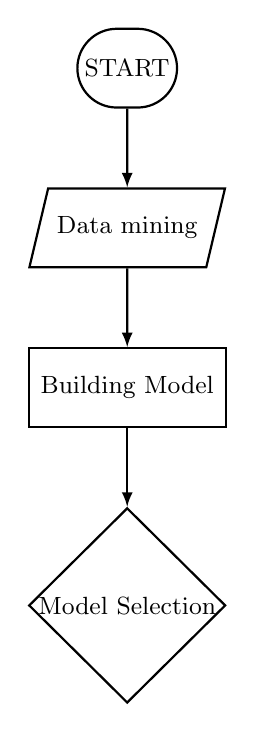
\begin{tikzpicture}[font=\small,thick]

        % Start block
        \node[draw,
            rounded rectangle,
            minimum width=1.5cm,
            minimum height=1cm] (block1) {START};
        
            
        % Voltage and Current Measurement
        \node[draw,
            trapezium, 
            trapezium left angle = 65,
            trapezium right angle = 115,
            trapezium stretches,
            below=of block1,
            minimum width=2.5cm,
            minimum height=1cm
        ] (block2) {Data mining};
        
        \node[draw,
            align=center,
            below=of block2,
            minimum width=2.5cm,
            minimum height=1cm
        ] (block3) {Building Model};
        
        
        \node[draw,
            diamond,
            below=of block3,
            minimum width=2.5cm,
            inner sep=0] (block4) {Model Selection};
        
       
        % Arrows
        \draw[-latex] (block1) edge (block2)
            (block2) edge (block3)
            (block3) edge (block4);
        
        \end{tikzpicture}
    \caption{Application Design}
    \label{fig:my_label}
\end{figure}
\mytodo{update the flowchart}

\subsection{Data Mining}
The most important aspect to train a complex system like is to feed adequate data set, so that model can perform well. However, the information required for preparing dataset is not readily available. In below sub sections the steps of Data mining is described. 
\subsubsection{Source Identification}\hspace*{\fill} \\
The subject matter experts are the first point of contact to identify the source to identify the suspicious companies. It is important to understand how traditionally the auditors, credit under taking team analyse the data and identify the key indicators. In the end of the day fraudulent transaction or activity is a human behaviour, hence the experts in this field look for particular patterns and indicators to identify the suspicious entity. The pattern in the financial transaction and general activities of the company are monitored to identify the patters. Below repetitive steps are taken to identify each key indicators.

\begin{enumerate}
    \item Make a comprehensive list of all possible indicators by taking notes from different subject matter experts. 
    \item Identify if there is any human biases on selected indicators  
    \item Determine if the identified variable is a binary (flag) or continues variable. 
    \item Identify the source of the data, i.e. internal source (financial statements, company profile) or external source. 
\end{enumerate}
\subsubsection{Data Extraction}\hspace*{\fill} \\
The next activity to prepare the training data set is to extract data from historical company information. Based on the selected key indicators the combines sources are identified. For the current problem its been found that majority of the information are coming from company financial information kept is a Oracle database and historical company reports which are kept in Extensible Markup Language (xml) format. For data extraction step all the indicators for past 10 years have been taken from these sources. The extracted information is kept in MongoDB server where the information of each companies are kept. The financial information are fetched from existing oracle DB, however the vital company information are extracted from the XML and kept in a JSON \mytodo{cite} format for further uses. 

\mytodo{Flow diagram needs to be added}

\subsubsection{Feature Engineering}\hspace*{\fill} \\
After the features extraction feature engineering is done to generate features based on the identified indicators. The engineered features are based on the financial information, company activities and recombination of the information. Due to sensitivity of the data, the details of the features are not mentioned. However below are the general overview of the feature engineering

\begin{itemize}
    \item \textbf{Financial:} The historical and recent financial information of each company have been collected. This data shows the trend and pattern of the company over last 10 years. During features extraction the anomalies are flagged and converted into a binary variable. There are lots of floating points information like yearly profit are kept as continues variable. 
    
    \item \textbf{Non Financial:} The non financial features are mainly based on the behavioural aspect of personal and the company. As the behavioural information is not easily transferable to features, the important activities and characteristics are marked and binary or continues variable. Information like trade sector, abnormal changes of company, vital dates, recent suspicious transactions etc. are engineered as features.
    
    \item \textbf{Combination:} It was noticed that some of the useful additional features can be mined using the combination method. In a combination method new feature can be created combining two or more financial or non financial features by using logical or mathematical process. For example a new marker can be created to find the ratio of number of employees and overall financial turnover of the company. 
\end{itemize}

below pseudo code structure [Algorithm :\ref{alg:feature}]is used to engineer features from extracted data . 

\begin{algorithm}
    \caption{Feature Engineering}
    \label{alg:features}

    \SetKwProg{feature}{Function \emph{feature}}{}{end}
    
        \feature{(Company Object)}{
            \textbf{Input:}{ company information in JSON formal} \\
            \textbf{Output:}{ feature value (int - flag, float for continues variable}
      
            \State {$feature\_counter \gets 0$ \CommentSty{Initialise the counter}} \\
            
            \If{ $report\_date$ is available}{
                  $important\_date$ = $report\_date$\;
              }
            \Else{}{\Return $feature\_counter$}
             
            \State {$json\_expression$ \= parse JSON to get feature information} \\
            \State{$list \gets$ value from $json\_expression$ }\\
           \\
            \ForAll{child $c$ in list}{
                \If{$important\_date \leq child['date']$ }{
                        $feature\_counter$ ++
                    }
                 
            }
            \Return $feature\_counter$\\
        }

\end{algorithm}


\subsubsection{Exploratory data analysis}\hspace*{\fill} \\

From the feature extraction and feature engineering stage we get the full data set. To prepare the dataset total last 10 years of data for all companies (having \mytodo{cla} date) are selected. Due to time complexity for data extraction and keep to understand only recent trend last 10 years data is considered. In the data set we can see the there are total 30 columns, however the number of features are 27. The total number of features are 48,549. Among this data only 1358 are marked fraudulent or suspicious company. The actual data is around 100k during this period. However to keep the data mining time low, the dataset size kept to 48,549. From the paper on SMOTE \cite{}, we have seen the under sampling with SMOTE performs re lately well. So theoretically the performance will still get improvement.
\begin{itemize}
    \item Total number of columns: 30
    \item Number of company entries: 48,539
    \item Target label: Fraudulent
    \item Total Features: 27
    \item Total Fraudulent / suspicious: 1358
\end{itemize}

From the initial assessment we can see the that classes are very imbalanced. In the dataset there is only 1358 fraudulent cases out of 48,549 ones. That means only 2.8\% of companies are fraudulent or specious. 

\begin{figure}[H]
    \centering
    \includegraphics[width=.8\linewidth]{figures/class_imbalance.png}
    \caption{Class Distribution}
    \label{fig:class distribution}
\end{figure}

The complexity to build a model to detect a huge obstacle. In the features \ref{fig:Dimension reduction}
\begin{figure}[H]
    \centering
    \includegraphics[width=\linewidth]{figures/pca_2d.png}
    \caption{Dimension reduction}
    \label{fig:Dimension reduction}
\end{figure}
The proportion of the fraudulent cases is shown in figure \ref{fig:feature proportion}. 
\begin{figure}[H]
    \centering
    \includegraphics[width=\linewidth]{figures/feature_proportion.png}
    \caption{Proportion of binary features}
    \label{fig:feature proportion}
\end{figure}

\begin{figure}[H]
    \centering
    \includegraphics[width=\linewidth]{figures/corr.png}
    \caption{Correlation Matrix}
    \label{fig:corr}
\end{figure}

\subsubsection{Dataset Finalisation}\hspace*{\fill} \\
Finally the dataset has been segmented into train and test sets. From the
\begin{itemize}
    \item \textbf{Train and test split:}
    \item \textbf{Data Pre-processing:}
    \item \textbf{Handle class Imbalance:}
\end{itemize}

\subsection{Model configuration}

\subsubsection{Random Forest}\hspace*{\fill} \\
Random forest algorithm generally performs better compare with other classification algorithms for imbalanced dataset \cite{Valecha2018PredictionOC}. In random forest model classifier ensemble different trees and final prediction happens by voting and selecting the majority decision. 

\begin{enumerate}
    \item Randomly select N number of Features
    \item Train a Decision Tree with selected features
    \item Select the target number of tress and repeat first two steps 
    \item Each tree predicts the class for new entry
    \item The final class prediction done by majority vote. 
\end{enumerate}

In our random forest,we set tree number to 200. We also use grid search method to set some ratio of the class weights and other related parameters to select the most suitable one with the highest accuracy. For example,the class weight selection process is shown in Fig.2. As the figure shows, when our weights equals to the ratio of 1:1 and 1:2, our accuracy perform best. Therefore, we set the class weight as 1:1 in the experiment.Also there are some other parameters we will not enumerate here but the process are the same. \mytodo{text needs to be updated}

\begin{figure}[htp]
    \centering
    \includegraphics[width=\linewidth]{}
    \begin{forest}
      for tree={l sep=3em, s sep=3em, anchor=center, inner sep=0.7em, fill=blue!50, circle, where level=2{no edge}{}}
      [
      Training Data, node box
      [sample and feature bagging, node box, alias=bagging, above=4em
      [,red!70,alias=a1[[,alias=a2][]][,red!70,edge label={node[above=1ex,red arrow]{}}[[][]][,red!70,edge label={node[above=1ex,red arrow]{}}[,red!70,edge label={node[below=1ex,red arrow]{}}][,alias=a3]]]]
      [,red!70,alias=b1[,red!70,edge label={node[below=1ex,red arrow]{}}[[,alias=b2][]][,red!70,edge label={node[above=1ex,red arrow]{}}]][[][[][,alias=b3]]]]
      [~~$\dots$~,scale=2,no edge,fill=none,yshift=-4em]
      [,red!70,alias=c1[[,alias=c2][]][,red!70,edge label={node[above=1ex,red arrow]{}}[,red!70,edge label={node[above=1ex,red arrow]{}}[,alias=c3][,red!70,edge label={node[above=1ex,red arrow]{}}]][,alias=c4]]]]
      ]
      \node[tree box, fit=(a1)(a2)(a3)](t1){};
      \node[tree box, fit=(b1)(b2)(b3)](t2){};
      \node[tree box, fit=(c1)(c2)(c3)(c4)](tn){};
      \node[below right=0.5em, inner sep=0pt] at (t1.north west) {Tree 1};
      \node[below right=0.5em, inner sep=0pt] at (t2.north west) {Tree 2};
      \node[below right=0.5em, inner sep=0pt] at (tn.north west) {Tree $n$};
      \path (t1.south west)--(tn.south east) node[midway,below=4em, node box] (mean) {mean in regression or majority vote in classification};
      \node[below=3em of mean, node box] (pred) {prediction};
      \draw[black arrow={5mm}{4mm}] (bagging) -- (t1.north);
      \draw[black arrow] (bagging) -- (t2.north);
      \draw[black arrow={5mm}{4mm}] (bagging) -- (tn.north);
      \draw[black arrow={5mm}{5mm}] (t1.south) -- (mean);
      \draw[black arrow] (t2.south) -- (mean);
      \draw[black arrow={5mm}{5mm}] (tn.south) -- (mean);
      \draw[black arrow] (mean) -- (pred);
    \end{forest}
    \caption{Random Forest}
    \label{fig:rand_forst_graph}
\end{figure}


\textbf{Hyper-parameter tuning:}
Random Forest classifiers comes with crucial parameters which needs to be tuned to get the best model. Below parameters are used in a random grid search method to do hyper parameter tuning for the random forest estimator. The options for each estimators are shown in the table: ~\ref{tab:RF_param}.
\begin{itemize}
    \item n\_estimator: Number of trees in random forest
    \item max\_features: Number of features to consider at every split
    \item max\_depth: Maximum number of levels in tree
    \item min\_samples\_split: Minimum number of samples required to split a node
    \item min\_sample\_leaf: Minimum number of samples required at each leaf node
    \item bootstrap: Method of selecting samples for training each tree
\end{itemize}

\begin{table}[h]
    \begin{tabular}{llll}
    Parameter           & Options         & No of options \\
    n\_estimator        & 200 to 2000     & 100           \\
    max\_features       & Auto, sqrt      & 2             \\
    max\_depth          & None, 10 to 110 & 12            \\
    min\_samples\_split & 2,5,10          & 3              \\
    min\_samples\_leaf  & 1,2,4           & 3              \\
    bootstrap           & True, False     & 2              \\
    \end{tabular}
    \caption{Hyper-parameter settings for Random Forest}
    \label{tab:RF_param}
\end{table}


\subsubsection{XDBoost}\hspace*{\fill} \\
\mytodo{Details of  XDBoost}
\subsubsection{Artificial Neural Network (ANN)}\hspace*{\fill} \\
\mytodo{Write the configuration of Neural network used}


\begin{table}[h] 
\begin{tabular}{lcc} 
Model: Model\_1 \\ \hline 
 Layer (type)                  & Output Shape                & Param \#    \\ \hline \hline 
 dense (Dense)                 & (None, 256)                 & 7168       \\ \hline 
 batch\_normalization (BatchNor &  (None, 256)                & 1024       \\ \hline 

 ormalization)                 &                             &            \\ \hline 
 dropout\_1 (Dropout)           & (None, 256)                 & 0          \\ \hline 
 dense\_2 (Dense)               & (None, 256)                 & 65792      \\ \hline 
 batch\_normalization\_2 (BatchN &  (None, 256)                & 1024       \\ \hline 

                               &                             &            \\ \hline \hline 
Total params: 142,081 \\ 
Trainable params: 140,545 \\ 
Non-trainable params: 1,536 \\ \hline 
\end{tabular} 
\caption{Model summary for ANN Model.} 
\label{tab:model-summary} 
\end{table}


\subsection{Method of Selection}
\mytodo{model selection hint\: https://medium.com/@matteding/imbalanced-data-fraud-detection-3185c1cdaa77}
\subsubsection{Confusion Matrix}\hspace*{\fill} \\
\mytodo{write how candonfusion matrix is used for model selection}
\subsubsection{AUC ROC}\hspace*{\fill} \\
\mytodo{how AUC ROC metrics are used}
\subsubsection{Threshold value}\hspace*{\fill} \\
\mytodo{Use of Threshold value to improve the model}
\section{Evaluation}\label{sec: Evaluation}
%Discuss the design of your experiments, the results you obtained,and how they help in evaluating the claims you made in the introduction. You may also use the evaluation results in this section to justify your design choices or assess the contributions of different aspects of your design towards the overall goals.

\subsection{Exploratory data analysis}\hspace*{\fill} \\

From the feature extraction and feature engineering stage we get the full data set. To prepare the dataset total last 10 years of data for all companies (having \mytodo{cla} date) are selected. Due to time complexity for data extraction and keep to understand only recent trend last 10 years data is considered. In the data set we can see the there are total 30 columns, however the number of features are 27. The total number of features are 48,549. Among this data only 1358 are marked fraudulent or suspicious company. The actual data is around 100k during this period. However to keep the data mining time low, the dataset size kept to 48,549. From the paper on SMOTE \cite{}, we have seen the under sampling with SMOTE performs re lately well. So theoretically the performance will still get improvement.
\begin{itemize}
    \item Total number of columns: 30
    \item Number of company entries: 48,539
    \item Target label: Fraudulent
    \item Total Features: 27
    \item Total Fraudulent / suspicious: 1358
\end{itemize}

From the initial assessment we can see the that classes are very imbalanced. In the dataset there is only 1358 fraudulent cases out of 48,549 ones. That means only 2.8\% of companies are fraudulent or specious. 

\begin{figure}[H]
    \centering
    \includegraphics[width=.8\linewidth]{figures/class_imbalance.png}
    \caption{Class Distribution}
    \label{fig:class distribution}
\end{figure}

The complexity to build a model to detect a huge obstacle. In the features \ref{fig:Dimension reduction}
\begin{figure}[H]
    \centering
    \includegraphics[width=\linewidth]{figures/pca_2d.png}
    \caption{Dimension reduction}
    \label{fig:Dimension reduction}
\end{figure}
The proportion of the fraudulent cases is shown in figure \ref{fig:feature proportion}. 
\begin{figure}[H]
    \centering
    \includegraphics[width=\linewidth]{figures/feature_proportion.png}
    \caption{Proportion of binary features}
    \label{fig:feature proportion}
\end{figure}

\begin{figure}[H]
    \centering
    \includegraphics[width=\linewidth]{figures/corr.png}
    \caption{Correlation Matrix}
    \label{fig:corr}
\end{figure}

\subsubsection{Dataset Finalisation}\hspace*{\fill} \\
Finally the dataset has been segmented into train and test sets. From the
\begin{itemize}
    \item \textbf{Train and test split:}
    \item \textbf{Data Pre-processing:}
    \item \textbf{Handle class Imbalance:}
\end{itemize}

According to results shown in [] AUC values are stable or increased using class imbalanced and data driven method. 

\mytodo{show figure for AUC curve}


\begin{table}[h]
\begin{tabular}{@{}|l|l|l|l|l|l|@{}}
\toprule
\textbf{PCA} & \textbf{SMOTE} & \textbf{Model} & \textbf{Accuracy} & \textbf{Precision} & \textbf{Recall} \\ \midrule
\multirow{6}{*}{No}  & \multirow{3}{*}{No}  & \textbf{RF} & 0.0000 & 0.0000 & 0.0000 \\ \cmidrule(l){3-6} 
                     &                      & \textbf{XD} & 0.0000 & 0.0000 & 0.0000 \\ \cmidrule(l){3-6} 
                     &                      & \textbf{NN} & 0.0000 & 0.0000 & 0.0000 \\ \cmidrule(l){2-6} 
                     & \multirow{3}{*}{Yes} & \textbf{RF} & 0.0000 & 0.0000 & 0.0000 \\ \cmidrule(l){3-6} 
                     &                      & \textbf{XD} & 0.0000 & 0.0000 & 0.0000 \\ \cmidrule(l){3-6} 
                     &                      & \textbf{NN} & 0.0000 & 0.0000 & 0.0000 \\ \midrule
\multirow{6}{*}{Yes} & \multirow{3}{*}{No}  & \textbf{RF} & 0.0000 & 0.0000 & 0.0000 \\ \cmidrule(l){3-6} 
                     &                      & \textbf{XD} & 0.0000 & 0.0000 & 0.0000 \\ \cmidrule(l){3-6} 
                     &                      & \textbf{NN} & 0.0000 & 0.0000 & 0.0000 \\ \cmidrule(l){2-6} 
                     & \multirow{3}{*}{Yes} & \textbf{RF} & 0.0000 & 0.0000 & 0.0000 \\ \cmidrule(l){3-6} 
                     &                      & \textbf{XD} & 0.0000 & 0.0000 & 0.0000 \\ \cmidrule(l){3-6} 
                     &                      & \textbf{NN} & 0.0000 & 0.0000 & 0.0000 \\ \bottomrule
\end{tabular}
\caption{Model performance over test set}
\label{tab:model performance}
\end{table}

\begin{table}
    \begin{tabular}{lrrr}
\toprule
{} &  a &  b &  c \\
\midrule
0 &  1 &  3 &  4 \\
1 &  4 &  5 &  6 \\
\bottomrule
\end{tabular}

    \caption{Demo results}
    \label{tab:results}
\end{table}


\subsection{Method of Selection}
\mytodo{model selection hint\: https://medium.com/@matteding/imbalanced-data-fraud-detection-3185c1cdaa77}
\subsubsection{Confusion Matrix}\hspace*{\fill} \\
\mytodo{write how candonfusion matrix is used for model selection}
\subsubsection{AUC ROC}\hspace*{\fill} \\
\mytodo{how AUC ROC metrics are used}
\subsubsection{Threshold value}\hspace*{\fill} \\
\mytodo{Use of Threshold value to improve the model}
\section{Discussion}\label{sec: discussion}
In this section, the discussion on the results presented in section~\ref{sec: Evaluation} is covered. The main discussion focuses on the performance comparison of each model. Based on section~\ref{sec: model results} of this report, the result discussion is covered. 

\subsubsection{Performance Metrics}\hspace*{\fill} \\
It is apparent from this table~\ref{tab:per_res} that accuracy for the models is not a suitable matrix. All the non SMOTE models got 97\% accuracy and for SMOTE models the accuracy varies from 86\% to 88\%. Considering the huge class imbalance we know even a naive model will give around 98\% accuracy. 

The results of precision metrics drop significantly from non-SMOTE to SMOTE models. In SMOTE models XGBoost has the highest precision rate of 0.44 and the artificial neural network has the lost rate of 0.30. For SMOTE group, the Random Forest model has the heights precision value of 0.11, which is significantly lower than the values in the no Smote group.   

The recall is a good matrix for imbalanced data set like this. In the table~\ref{tab:per_res} we can see that the recall performance of the models' increases from SMOTE than non SMOTE group. Random Forest and XGBoost with SMOTE have a heights recall score of 0.47. 

We see the f-1 score remain unchained for the artificial neural network. The f1-score improves significantly for XGBoost from 0.06 to 0.17 after SMOTE transformation. Random Forst with SMOTE also has a heights score of 0.17 which increase by .6 points. 


In the figure~\ref{fig:test_train} we can see that as expected the performances of all the model drops from train set to test set. The random forest model has the highest value (more than 0.8) in the train set, however, the performance dramatically drops for the test data. Similarly, ANN performs well in the train set however the performance test drops but not as much as random forest. The XGBoost performs the worst in both train and test data. From this chart, we can see the XGBoost and Random Forest with SMOTE performs well in the test dataset. 


\subsubsection{ROC Curves}\hspace*{\fill} \\
The results of the ROC curves are shown in figure~\ref{fig:roc_all}and in figure~\ref{fig:roc_all_2}. ROC curves give the idea of how the model performs for True Positive (TF) and False Positive (FP) cases. The no skill line shows us the guideline for the comparison of the models. From the figures, we can see that Random Forest with SMOTE appears to have the best ROC curve. On the other hand, XGBoost which looked promising in the table ~\ref{tab:per_res} completely fails the ROC curve tests. We can see the results gradually increases till 0.2, however, then it hardly performs any better than no skill models. The rest of the models perform similar to each other. 


\subsubsection{AUC ROC}\hspace*{\fill} \\
From the ROC curve analysis, we already got the Idea that the Random Forest with SMOTE performs the best. However, besides the XGBoost with SMOTE, most of the models' performance looks similar. The rest of the models' seems to have a similar area like Random Forest, hence checking the area under the curve by AUC ROC metrics is a good way for this scenario. In table~\ref{tab: roc_auc} we can see that Random Forest with SMOTE has the highest ROC AUC score of 0.817. XGBoost with SMOTE has the lowest 0.549 which is just a little better than the no skill model. The rest of the models as found in the ROC analysis have similar ROC AUC values starting from 0.693 to 0.793.


After analysing all the matrices we can say that the Random Forest with SMOTE performs the best among all the models. However, the overall performance of all the models is quite low. In the confusion matrix for our best model Random Forest with SMOTE, in the figure~\ref{fig:cm_rf}, we can see that only 213 suspicious cases were properly classified. The model fails to detect 164 cases and also gives a high false-positive case of 2999. After changing the threshold values, figure~\ref{fig:cm_rf_full} we can see that models tend to perform better, however, after the 0.4 threshold value, the models get a huge number of false positives. This is a clear indication that there is a scope of improvements. 
\section{Conclusion}\label{sec: conclusion}
% inital part of the conclusion



% additional points
Trade fraud is not only causes Economic damage to the business and their respective financial institutions, but also creates disrupt in the overall economy. Sometimes fraudulent companies use the fund for terrorism, human rights violation, money laundering.
\section{Future Work}\label{sec:future-work}

\begin{itemize}
    \item Deep sampling method can be applied 
    \item Genetic algorithm 
    \item Other types of neural networks like CNN, transformers 
\end{itemize}


\newpage
\appendix
\section{Appendix}\label{sec:appendix}

\hspace*{5cm}
\subsection{ROC Curves}
\begin{figure}[H]
    \centering
    \includegraphics[width=\linewidth]{figures/roc_res_full.PNG}
    \caption{ROC Curves }
    \label{fig:ROC_full_APX}
\end{figure}

\hspace*{5cm}
\subsection{Confusion Matrix}
\begin{figure}[H]
    \centering
    \includegraphics[width=\linewidth]{figures/cm_rf_th.PNG}
    \caption{Confusion Matrix - Random Forest with threshold values}
    \label{fig:cm_rf_full}
\end{figure}


\hspace*{25cm}
\subsection{Neural Network Training}
\begin{figure}[H]
    \centering
    \includegraphics[width=\linewidth]{figures/nn_training.PNG}
    \caption{Neural Network Training}
    \label{fig:cm_rf_full}
\end{figure}


\newpage
\addcontentsline{toc}{section}{References}
% \bibliographystyle{ACM-Reference-Format}
% \bibliography{ref.bib}
% \addbibresource{}
\printbibliography

\end{document}
